\documentclass[final]{beamer}\usepackage[]{graphicx}\usepackage[]{color}
%% maxwidth is the original width if it is less than linewidth
%% otherwise use linewidth (to make sure the graphics do not exceed the margin)
\makeatletter
\def\maxwidth{ %
  \ifdim\Gin@nat@width>\linewidth
    \linewidth
  \else
    \Gin@nat@width
  \fi
}
\makeatother

\definecolor{fgcolor}{rgb}{0.345, 0.345, 0.345}
\newcommand{\hlnum}[1]{\textcolor[rgb]{0.686,0.059,0.569}{#1}}%
\newcommand{\hlstr}[1]{\textcolor[rgb]{0.192,0.494,0.8}{#1}}%
\newcommand{\hlcom}[1]{\textcolor[rgb]{0.678,0.584,0.686}{\textit{#1}}}%
\newcommand{\hlopt}[1]{\textcolor[rgb]{0,0,0}{#1}}%
\newcommand{\hlstd}[1]{\textcolor[rgb]{0.345,0.345,0.345}{#1}}%
\newcommand{\hlkwa}[1]{\textcolor[rgb]{0.161,0.373,0.58}{\textbf{#1}}}%
\newcommand{\hlkwb}[1]{\textcolor[rgb]{0.69,0.353,0.396}{#1}}%
\newcommand{\hlkwc}[1]{\textcolor[rgb]{0.333,0.667,0.333}{#1}}%
\newcommand{\hlkwd}[1]{\textcolor[rgb]{0.737,0.353,0.396}{\textbf{#1}}}%
\let\hlipl\hlkwb

\usepackage{framed}
\makeatletter
\newenvironment{kframe}{%
 \def\at@end@of@kframe{}%
 \ifinner\ifhmode%
  \def\at@end@of@kframe{\end{minipage}}%
  \begin{minipage}{\columnwidth}%
 \fi\fi%
 \def\FrameCommand##1{\hskip\@totalleftmargin \hskip-\fboxsep
 \colorbox{shadecolor}{##1}\hskip-\fboxsep
     % There is no \\@totalrightmargin, so:
     \hskip-\linewidth \hskip-\@totalleftmargin \hskip\columnwidth}%
 \MakeFramed {\advance\hsize-\width
   \@totalleftmargin\z@ \linewidth\hsize
   \@setminipage}}%
 {\par\unskip\endMakeFramed%
 \at@end@of@kframe}
\makeatother

\definecolor{shadecolor}{rgb}{.97, .97, .97}
\definecolor{messagecolor}{rgb}{0, 0, 0}
\definecolor{warningcolor}{rgb}{1, 0, 1}
\definecolor{errorcolor}{rgb}{1, 0, 0}
\newenvironment{knitrout}{}{} % an empty environment to be redefined in TeX

\usepackage{alltt}
\usefonttheme{serif}
\mode<presentation>{\usetheme{ASU3}}
\usepackage{amsmath, amsfonts, amssymb, pxfonts, eulervm, xspace, enumerate, hyperref, color, bookmark}
\usepackage{graphicx}
\usepackage[orientation=landscape, size=custom, width =152.4, height=106.68, scale=1.4, debug]{beamerposter}
% \usepackage{natbib}

\usecolortheme{rose}
%\setbeamercolor{background canvas}{bg=magenta!16!yellow!90}

\beamertemplategridbackground[1cm]

%-- Header and footer information ----------------------------------
\newcommand{\footright}{\href{https://github.com/alanarnholt/USFS/}{https://github.com/alanarnholt/USFS/}}
\newcommand{\footleft}{\href{mailto:arnholtat@appstate.edu}{Faculty Advisors: Eric Marland \& Alan Arnholt}}

\def\conference{The Conference Name Here}
\title{Analyzing and Influencing Carbon Sequestration}
\author{Ben Jones, Hannah X Laws, Andrew Sullivan, Kelly Loucks} 
\institute{Department of Mathematical Sciences}
%-------------------------------------------------------------------


%-- Main Document --------------------------------------------------
\IfFileExists{upquote.sty}{\usepackage{upquote}}{}
\begin{document}
\begin{frame}[fragile]
\vspace{-2ex}
\begin{columns}[t]





%%%%%%%%%%%%%%%%%%%%%%%%%%%%%%%%%%%%%%%%%%%%%%%%%%%%%%%%%%%%%%%%%%%
%-- Column 1 ---------------------------------------------------
\begin{column}{0.23\linewidth}
\begin{minipage}[t][.955\textheight]{\linewidth} 

%-- Block 1-1
\vspace{0ex}
\begin{block}{Abstract}
Sequestration of carbon in forests is a process that can pull large quantities of carbon out of the atmosphere or prevent its release to the atmosphere, 87\% of total CO2 removals in 2014. Carbon mitigation efforts have thus focused much attention on reforestation, forest management,and forest based products.  According to the most recent report to the UNFCCC, an estimated 18.7\% of the total carbon in woody materials is contained in harvested wood (HWP and SWDS).  
\vspace{2ex}
The amount of carbon in HWP and SWDS depend on how much wood is harvested, what types of products are produced, how the products are used, the lifetime of the wood products, and how the wood is processed at the end of its primary product lifetime.

\vspace{0ex}
\end{block}
\vfill

%-- Block 1-2
\begin{block}{Carbon Contributions}
\begin{itemize}
\item In 2005, the contribution to removals was 30 Tg (million metric tons) C (carbon) and 31 Tg C for the Production and Atmospheric Flow Approaches, respectively, and 44 Tg C for the Stock Change Approach. This range is 17 to 25 percent of C removals by forests, or would offset 42 percent to 61 percent of residential natural gas C emissions in 2005. 
\vspace{1ex}
\item The contribution has declined under the Production and Atmospheric Flow Approaches since 1990 and has increased under the Stock Change Approach. The Stock Change estimate has increased because it explicitly includes C in increasing net imports of wood and paper products. 
\vspace{1ex}
\item The contribution estimates were validated by adjusting the half-life of products in use in order to match independent estimates of carbon in housing in 2001 and annual wood and paper discards to solid-waste disposal sites (SWDS) during 1990 to 2001. Estimates of methane emissions from wood and paper in landfills were also checked against independent estimates of total landfill methane emissions. 

\end{itemize}
\vspace{0ex}
\vfill
\end{block}
\vfill

%-- Block 1-3
\begin{block}{Sources of Data and Equations}

\begin{enumerate}[I.]
\item WOODCARB II Software in Microsoft Excel\textsuperscript{\textregistered}
\vspace{0ex}
Note: Base level data was given in spreadsheet. 
\item Harvest Quantities:
\item Imports, Exports, etc.:
\item Decay of HWP:
\end{enumerate}
\vspace{0ex}

\end{block}
\vfill

%-- Block 1-4

\begin{block}{Accounting Approaches}

\begin{itemize}
\item International workshops identified three approaches to re- port HWP contribution. These approaches focus on account- ing differently for changes in carbon in HWP imports and exports.
\item Stock Change:
\item Production:
\item Atmospheric Flow:
\end{itemize}


\end{block}
\vfill

%-- Block 1-5

\begin{block}{Access to Packages}

\begin{enumerate}
\item Our incredible \href{http://madeitup.com}{web page}
\item Our incredible \href{http://benjones2.github.io/WOODCARB3R/}{WOODCARB3R package}
\end{enumerate}


\end{block}
\vfill

\end{minipage}
\end{column}%1

%%%%%%%%%%%%%%%%%%%%%%%%%%%%%%%%%%%%%%%%%%%%%%%%%%%%%%%%%%%%%%%%%
%-- Column 2 ---------------------------------------------------

\begin{column}{0.23\linewidth}
\begin{minipage}[t][.955\textheight]{\linewidth} 

%--Block 2-2 
\begin{block}{Purpose}
\vspace{0ex}
\begin{itemize}
\item Information is intended to aid in international discussions and any agreements about managing greenhouse gas emissions and sinks.
\item Also providing national level methods and estimates of carbon sinks and emissions associated with HWP.
\item
\end{itemize}
\vspace{-1.5ex}
\end{block}
\vfill


%-- Block 2-2
\vspace{0ex}
\begin{block}{Sensitvity Analysis}
\begin{itemize}
\item Used to determine how different values of an independent variable impact a particular dependent variable under a given set of assumptions. 
\item How the uncertainty in the output of a mathematical model or system can be apportioned to different sources of uncertainty in its inputs.
\item Helps in identifying the key variables that are major influence in the cost and benefits of the project.
\item 
\end{itemize}
\vspace{0ex}
\end{block}
\vfill

%-- Block 2-3
\begin{block}{Methods for Analyzing Sensitivity}
\begin{itemize}
\item A Monte-Carlo simulation used to assess the effect of uncertainty in inputs suggests the 90 percent confidence interval for removal contribution estimates under the three approaches is within –23\% to +19\%.
\vspace{2ex}
\item Monte Carlo simulation is a computerized mathematical technique that allows people to account for risk in quantitative analysis and decision making.
\item
\item
\end{itemize}
\vspace{0ex}
\vfill
\end{block}
\vfill

%-- Block 2-4
\begin{block}{Results}

\begin{enumerate}[I.]
\item Overall:


\item Susceptible Variables:


\item Discussion:


\end{enumerate}
\vspace{0ex}

\end{block}
\vfill


\end{minipage}
\end{column}%2

%%%%%%%%%%%%%%%%%%%%%%%%%%%%%%%%%%%%%%%%%%%%%%%%%%%%%%%%%%%%%%%%%%
%--Column 3 ----------------------------------------------------

\begin{column}{0.23\linewidth}
\begin{minipage}[t][.955\textheight]{\linewidth} 

%-- Block 3-1
\vspace{0ex}
\begin{block}{Current Analysis}
\vspace{0ex}
\begin{itemize}
\item
\item
\item
\item
\end{itemize}
\vspace{0ex}
\end{block}
\vfill

%-- Block 3-2
\begin{block}{Future Predictions}
\begin{itemize}
\item
\item
\item
\item
\end{itemize}
\vspace{0ex}
\vfill
\end{block}
\vfill

%-- Block 3-3
\vspace{0ex}
\begin{block}{Graph}
\vspace{0ex}
\begin{figure}
  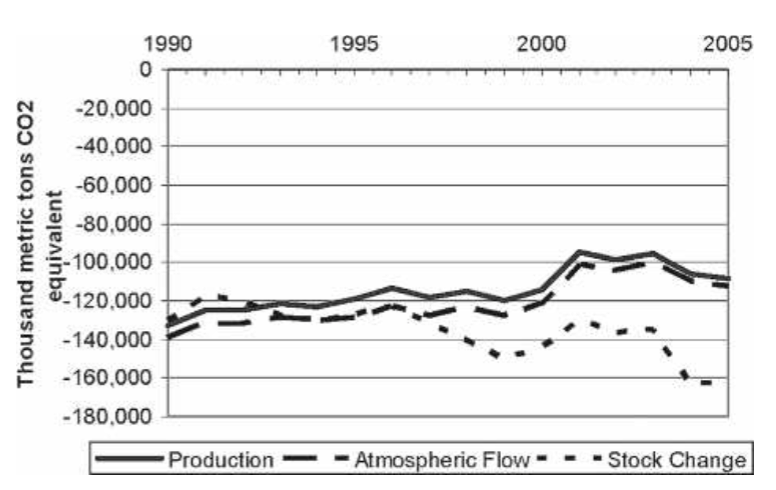
\includegraphics[width=\linewidth]{graph1.png}
  \caption{Harvested wood product contribution to forest sinks and emissions by approach – Gg CO2/ yr.}
  \label{Figure 1}
\end{figure}
\vspace{0ex}
\end{block}
\vfill

%-- Block 3-4
\vspace{0ex}
\begin{block}{Graph}
\vspace{0ex}

\vspace{0ex}
\end{block}
\vfill

\end{minipage}
\end{column}%3

%%%%%%%%%%%%%%%%%%%%%%%%%%%%%%%%%%%%%%%%%%%%%%%%%%%%%%%%%%%%%%%%
%-- Column 4 ---------------------------------------------------
\begin{column}{0.23\linewidth}
\begin{minipage}[t][.955\textheight]{\linewidth} 

%-- Block 4-1
\vspace{0ex}
\begin{block}{Potential Strategies}
\vspace{0ex}
\begin{itemize}
\item
\item
\item
\item
\end{itemize}
\vspace{0ex}
\vfill
\end{block}
\vfill

%-- Block 4-2
\begin{block}{Conclusions}
\begin{itemize}
\item
\item
\item
\end{itemize}
\vspace{0ex}
\vfill
\end{block}
\vfill

%-- Block 4-3
\begin{block}{Possible Extensions}
\begin{itemize}
\item  
\item  
\item  
\end{itemize}
\vspace{0ex}
\vfill
\end{block}
\vfill

%-- Block 4-4
\begin{block}{References}
\footnotesize
\setbeamertemplate{bibliography item}[text]
\vspace{-1ex}


\bibliographystyle{plain}  % can use plain but comment out natbib at top if using plain
\bibliography{knitr-packages,poster}
\normalsize
\vfill
\end{block} 
\vfill

\end{minipage}
\end{column}%4




\end{columns}
\end{frame}
\end{document}

